\section{Induktion, Rekursion, Kardinalität (33ff)}
Beweisprinzip der vollständigen Induktion. Rekursive Definition. Summationssymbol. Produktsymbol. Formel für (endliche) geometrische Summen. Definition von endlich, unendlich, abzählbar. 

\subsection{Beweisprinzip der vollständigen Induktion (34)}
Induktionsverankerung ($n=1$): Für $n=1$ ergibt sich die Aussage \textbf{TBD} welche wahr ist. Für den
Induktionsschritt sei $n\in\mathbb{N}$. Unter Annahme der Induktionsvoraussetzung \textbf{TBD (1)}, erhält man
\textbf{TBD} was zeigt, dass die Aussage auch für $n+1$ gilt und somit den Induktionsbeweis abschließt.

\begin{itemize}
\item \textbf{IA} $n=1$
\item \textbf{IV} 
\item \textbf{IS} $n \rightarrow n+1$
\end{itemize}

\subsection{Rekursive Definition (36)}
z.B. Fibonacci-Folge
\begin{equation}
\begin{split}
(a_n)_{n \in \mathbb{N}} &= a_{n-1} + a_{n-2} \\ 
a_0 &= 0 \\
a_1 &= 1
\end{split}
\end{equation}

\subsection{Summationssymbol (38)}
\begin{equation}
\begin{split}
\sum\nolimits_{i=1}^1 a_i &:= a_i \\
\sum\nolimits_{i=1}^{n+1} a_i &:=  a_i + \sum\nolimits_{i=1}^{n} \text{für } n \geq 1
\end{split}
\end{equation}

\subsection{Produktsymbol (39)}
\begin{equation}
\begin{split}
\prod\nolimits_{i=1}^1 a_i &:= a_i \\
\prod\nolimits_{i=1}^{n+1} a_i &:= a_i * \prod\nolimits_{i=1}^{n} \text{für } n \geq 1
\end{split}
\end{equation}


\subsection{Formel für (endliche) geometrische Summen (40)}
\begin{figure}[H]
	\centering
  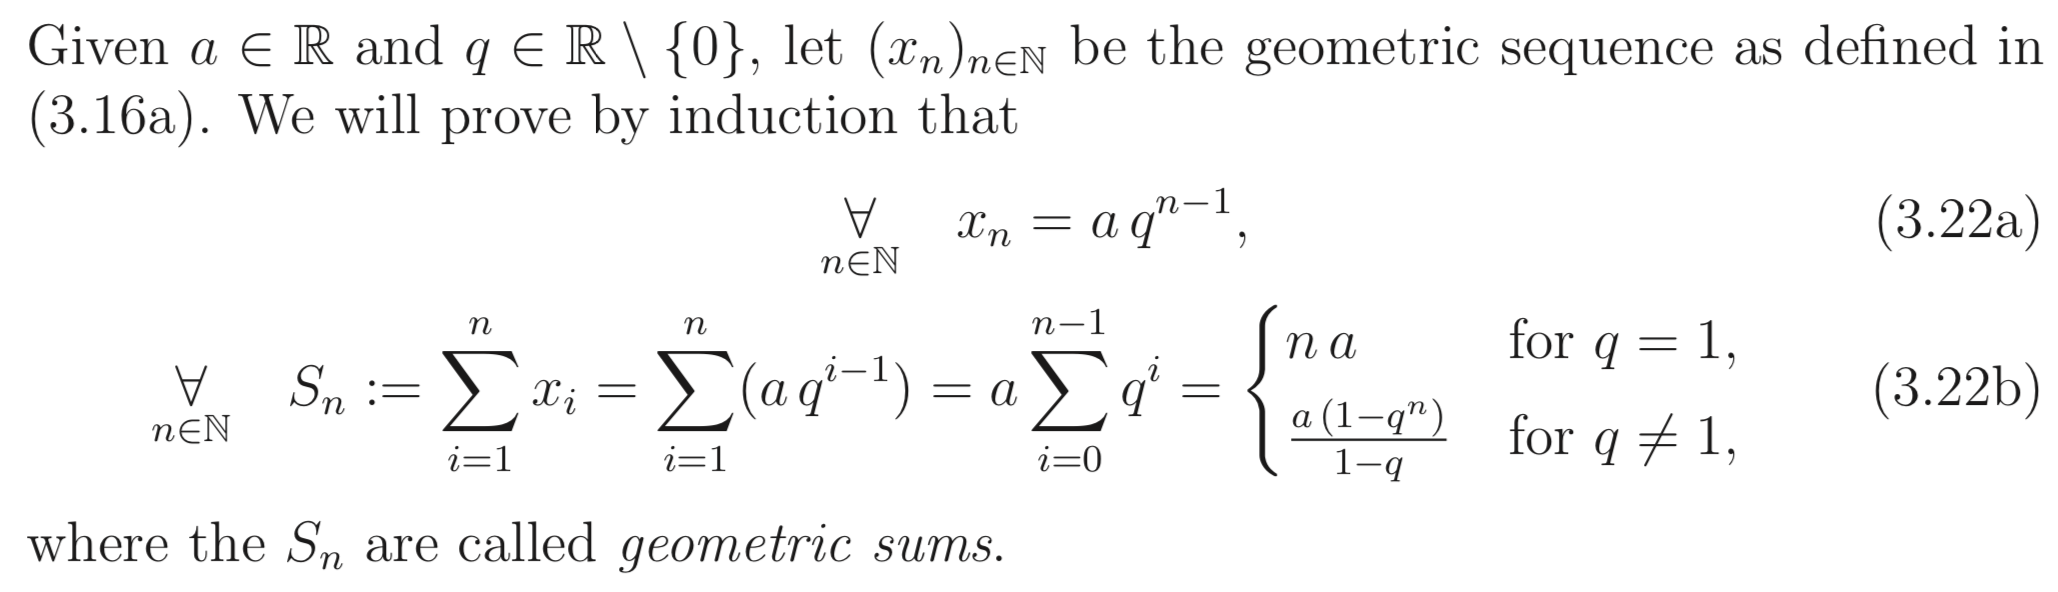
\includegraphics[width=0.7\textwidth]{media/40-example-3-11b.png}
	\caption{40 example 3.11b}
	\label{40_example_3.11b}
\end{figure}

\subsection{Definition von endlich, unendlich, abzählbar (40f)} 
Die Menge $A$ lautet
\begin{itemize}
\item endlich $\Leftrightarrow$ $\exists n \in \mathbb{N_0}$ sodass $\#A = n$ ($\#A :=$ Kardinalität, Anzahl Elemente in $A$)
\item unendlich $\Leftrightarrow$ $A$ ist nicht endlich. ($\#A = \infty$)
\item abzählbar $\Leftrightarrow$ $A$ ist endlich oder $\#A = \#\mathbb{N}$
\end{itemize}
